\chapter{Interfaces and Validation}
\section{Interface Overview}
The React application provides authenticated pages for anomalies, risk, login logs, and AI investigation. Administrator navigation additionally exposes the global dashboard, directory, and audit views. Backend authorization remains authoritative.

Login and registration operate outside the protected layout. Authentication context retains the token and safe user data in local storage; the shared client attaches the bearer token and clears session state after relevant unauthorized responses. Directory controls change account state, while the audit view and browser console serve separate security-record and diagnostic purposes.

Anomaly filters expose rule type, severity, and event context. Risk summarizes the preceding 24 hours; login views expose underlying records and administrator-created demonstration events. The AI workspace selects investigator, operator, or collaborative behavior and submits prompt, context, steering, and follow-up arrays. Its trace displays returned tool outcomes.

\clearpage\section{Application Screenshots}
Six captures were selected to show the entry point, overall monitoring, event investigation, personal account scope, and AI workspace. They are reproduced from candidate-provided screenshots without changing the displayed content. Counts and scores describe the captured demonstration state, not evaluation results.

\begin{figure}[!ht]\centering
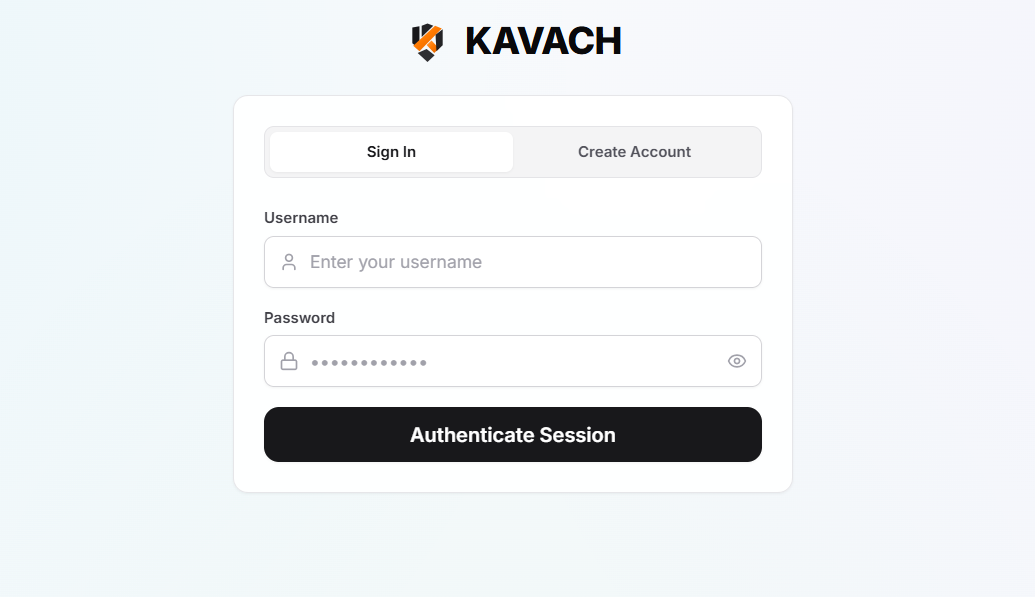
\includegraphics[width=.75\textwidth]{images/screenshot-login.png}
\caption{Sign-in interface with account-registration tab and authentication form.}\label{fig:screen-login}
\end{figure}

\begin{figure}[!ht]\centering
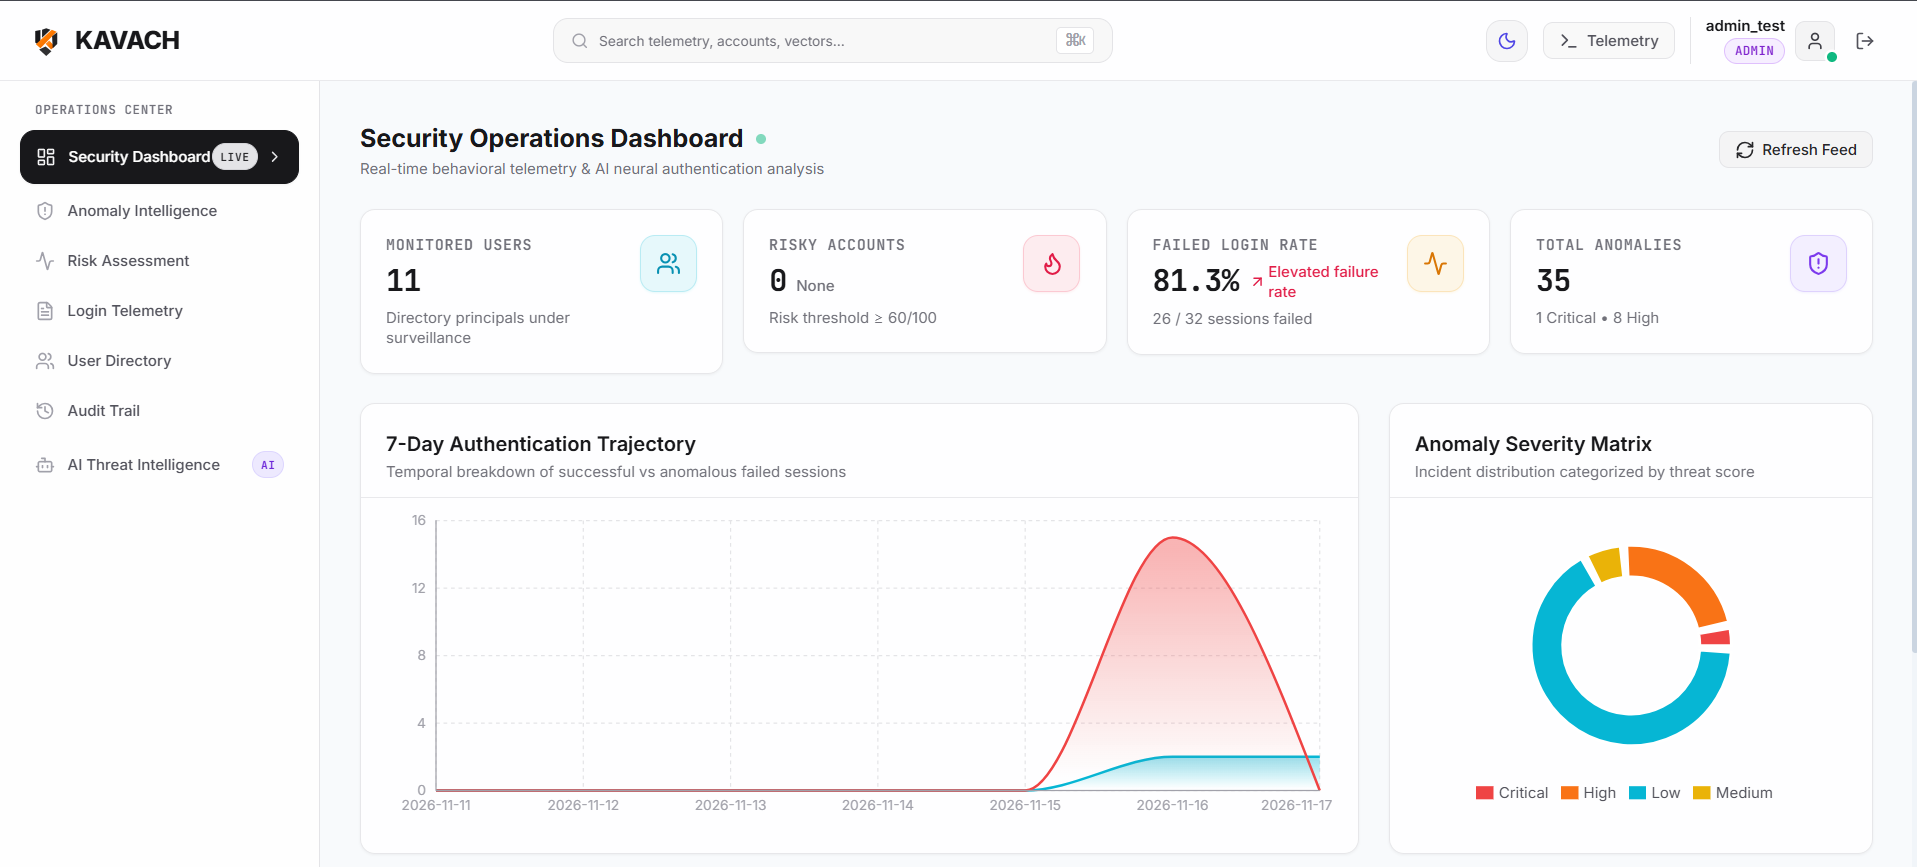
\includegraphics[width=\textwidth]{images/screenshot-dashboard.png}
\caption{Administrator dashboard: account counts, login outcomes, trend, and anomaly severity.}\label{fig:screen-dashboard}
\end{figure}

\clearpage\subsection{Anomaly Investigation and Login Telemetry}
The anomaly view exposes rule matches and per-alert weights, while the telemetry view shows the underlying login-event fields. Filters and action buttons are visible entry points; the captures do not show the outcomes of clicking those actions.

\begin{figure}[!ht]\centering
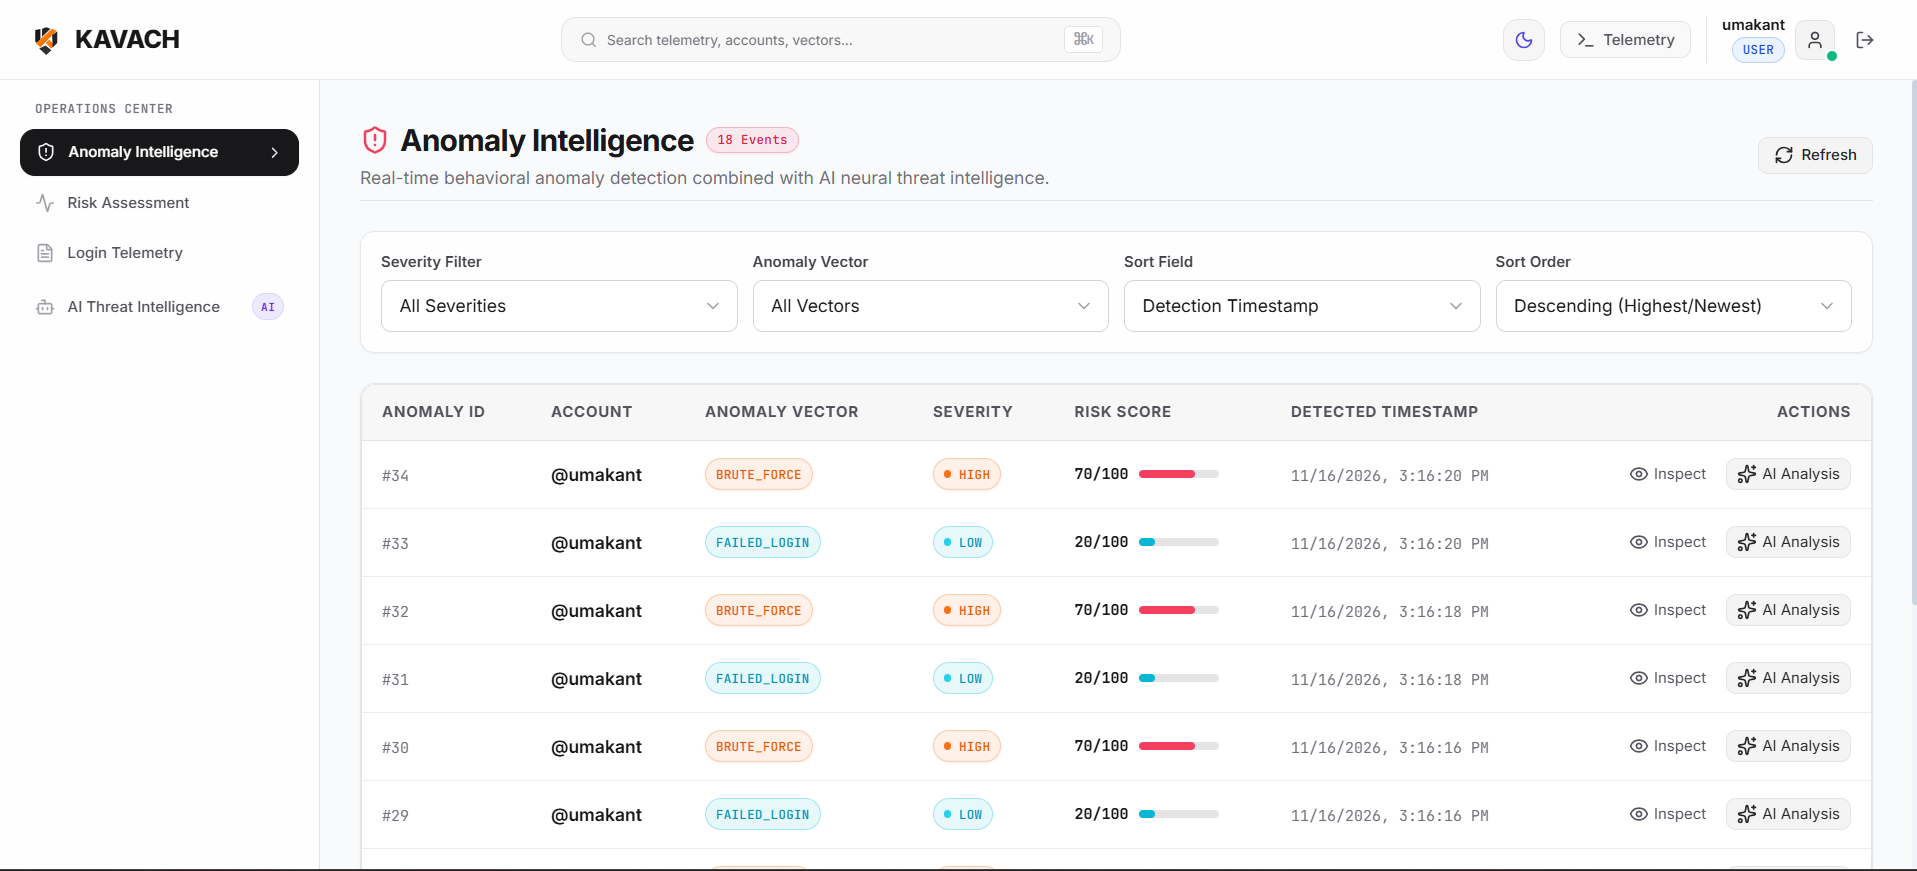
\includegraphics[width=\textwidth]{images/screenshot-anomalies.png}
\caption{User-scoped anomaly list with filters, rule types, severity, and alert weights.}\label{fig:screen-anomalies}
\end{figure}

\begin{figure}[!ht]\centering
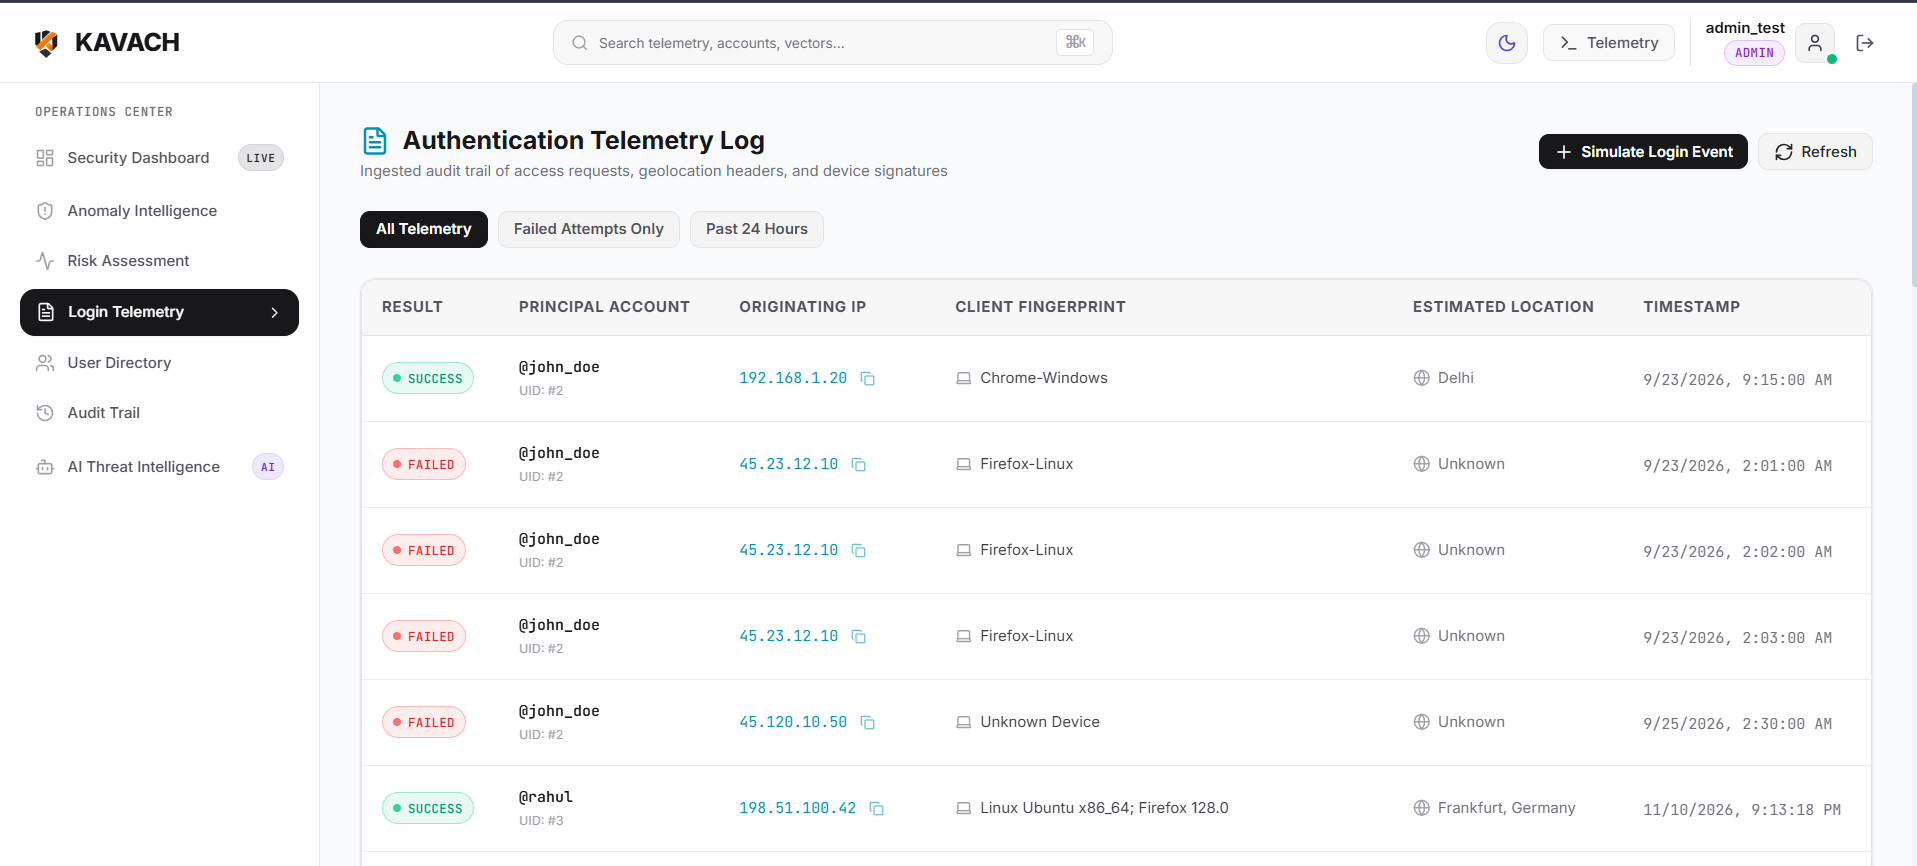
\includegraphics[width=\textwidth]{images/screenshot-telemetry.png}
\caption{Login telemetry showing successful and failed events with account and client metadata.}\label{fig:screen-telemetry}
\end{figure}

\clearpage\subsection{Personal Risk and AI Workspace}
The personal view displays the signed-in account's risk profile. Historical anomaly counts and the recent 24-hour risk score use different horizons. Interface subtitles such as ``Bayesian'' or ``neural'' do not alter the fixed-rule detector and additive score documented in Chapter 4. The AI capture shows its initial console state rather than a completed model or tool execution.

\begin{figure}[!ht]\centering
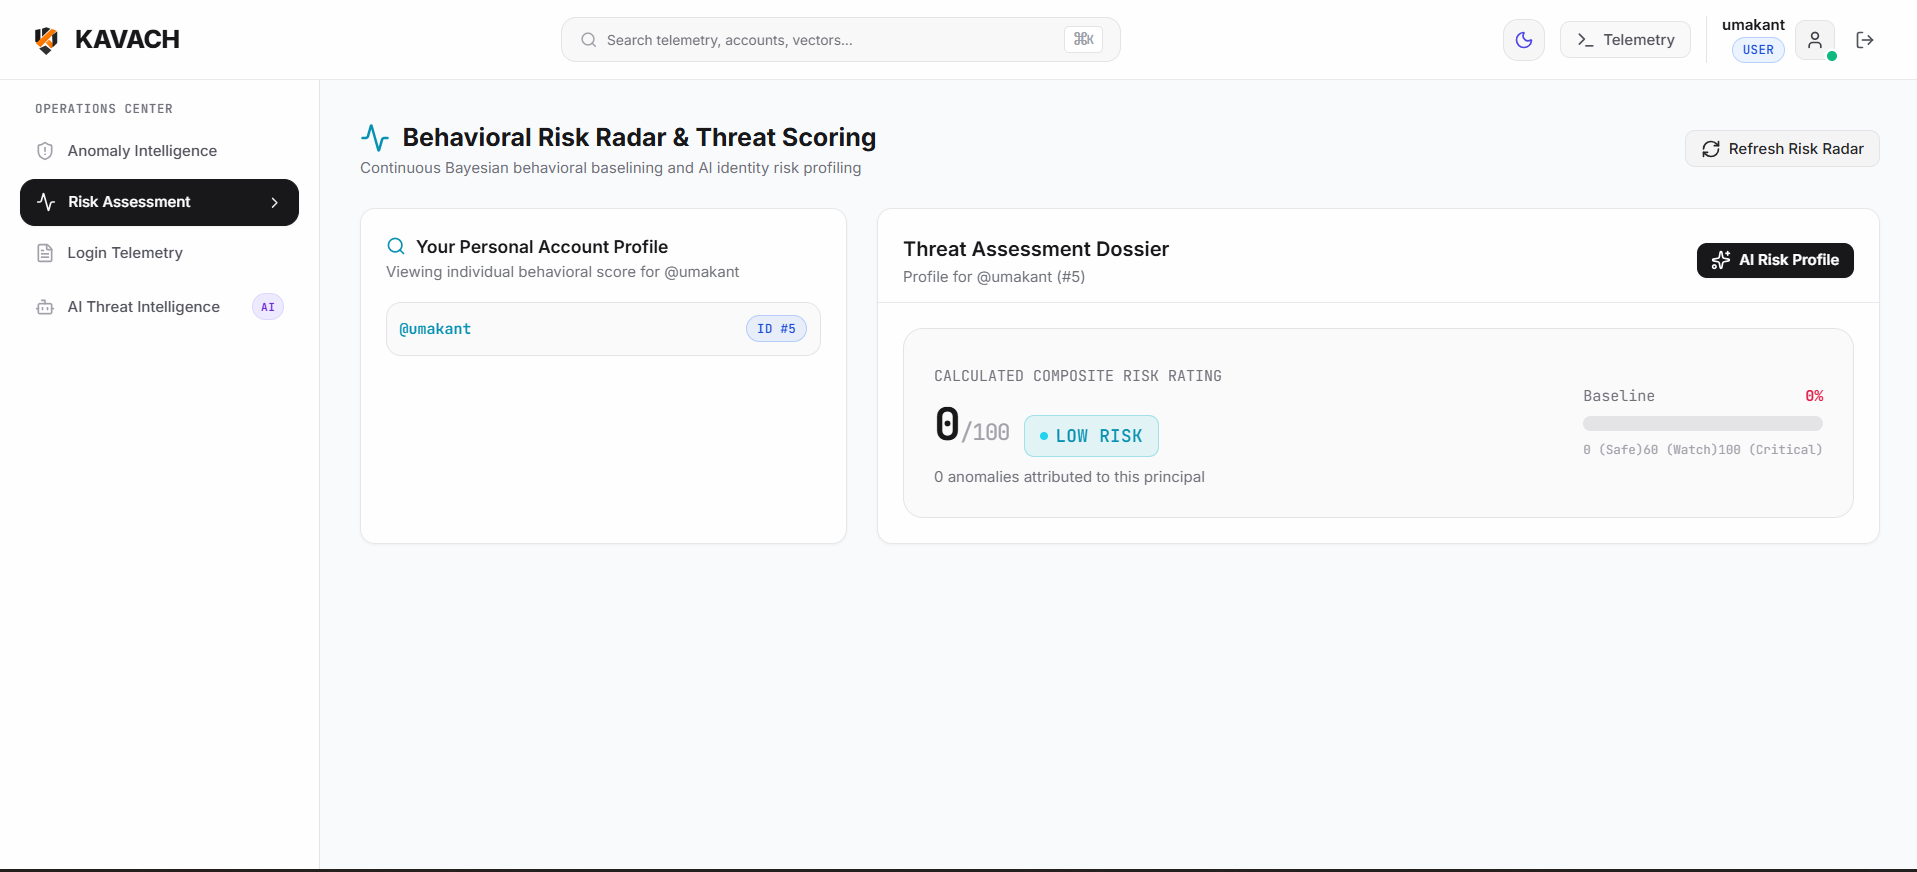
\includegraphics[width=\textwidth]{images/screenshot-personal-risk.png}
\caption{Personal risk view for the USER account, showing the displayed score and profile.}\label{fig:screen-risk}
\end{figure}

\begin{figure}[!ht]\centering
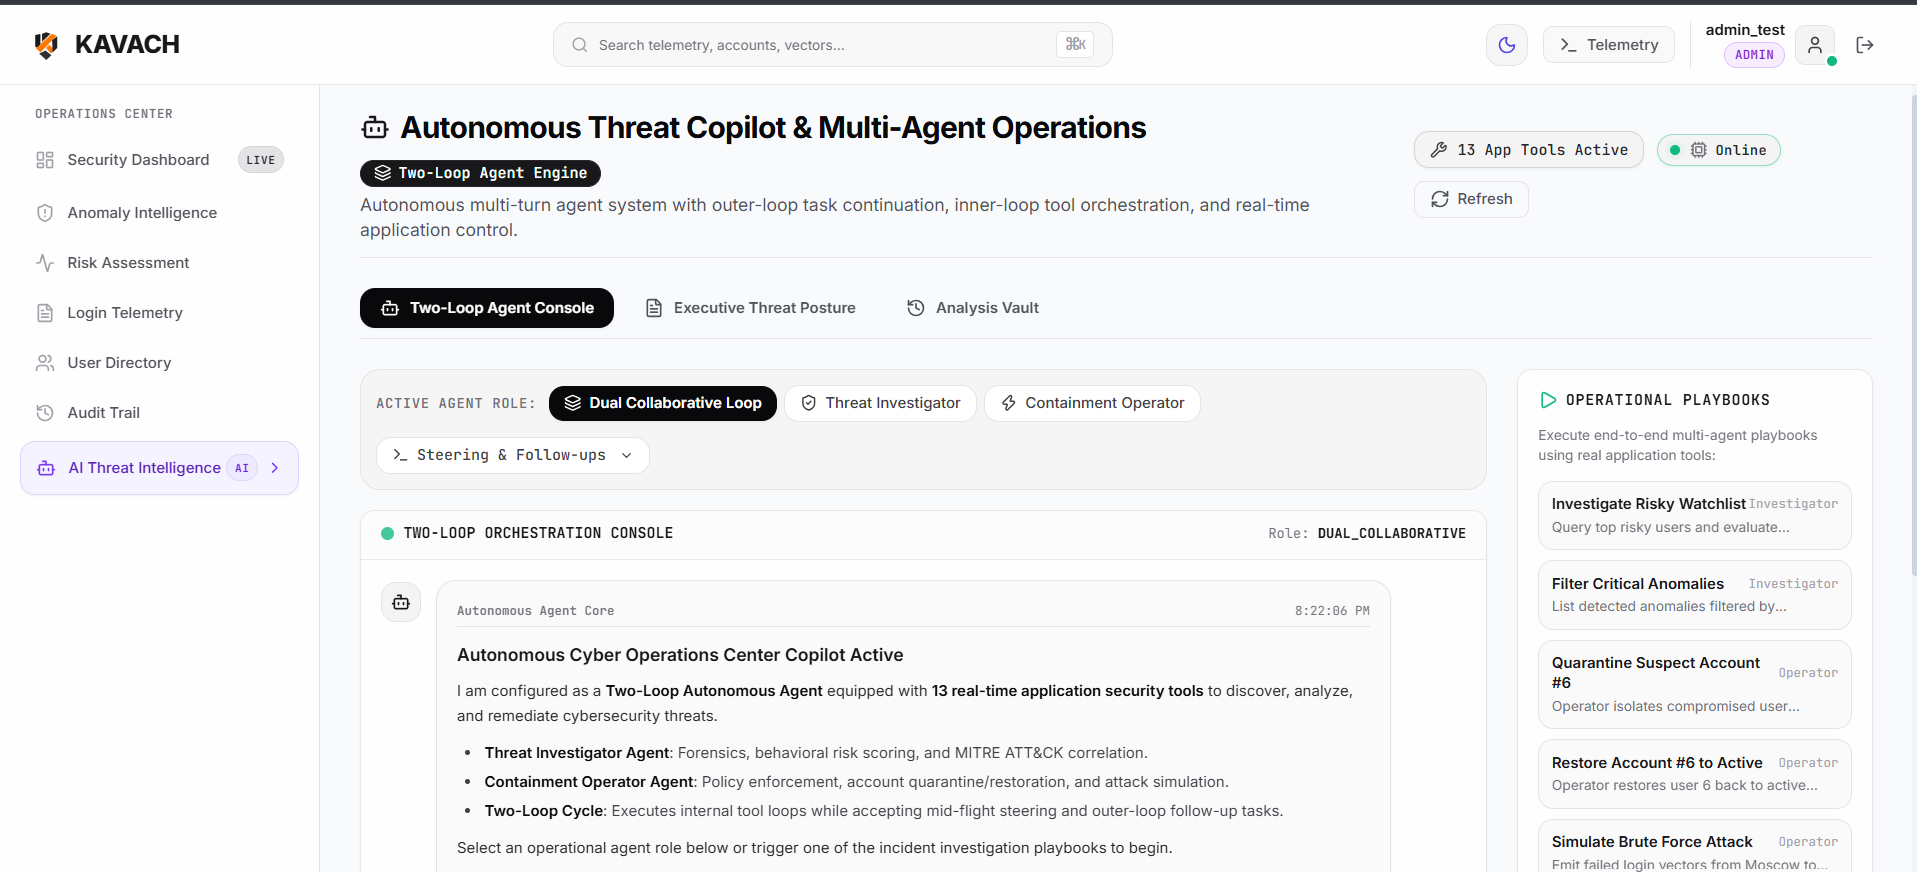
\includegraphics[width=\textwidth]{images/screenshot-ai-console.png}
\caption{AI workspace with agent-role selection, a 13-tool indicator, and operational playbooks.}\label{fig:screen-ai}
\end{figure}


\clearpage\section{Validation Plan}
The candidate's screenshots document visible interface states. The repository includes a context-loading test, but no controlled rule-test or load-test results were supplied. Table~\ref{tab:tests} lists expected outcomes to verify, not recorded passes.
\begingroup\footnotesize\setstretch{1.0}\renewcommand{\arraystretch}{1.1}\setlength{\parskip}{0pt}
\begin{longtable}{>{\raggedright\arraybackslash}p{0.9cm}>{\raggedright\arraybackslash}p{6.1cm}>{\raggedright\arraybackslash}p{7cm}}
\caption{Functional validation plan; execution pending.}\label{tab:tests}\\\toprule ID & Input / action & Expected behavior to verify\\\midrule\endfirsthead
\toprule ID & Input / action & Expected behavior to verify\\\midrule\endhead
T1 & Register unique credentials. & Active USER, encoded password, safe response, audit event.\\
T2 & Repeat username or email. & Conflict and no duplicate account.\\
T3 & Valid password for active user. & JWT, success telemetry, applicable contextual rules.\\
T4 & Incorrect password for known user. & Unauthorized; failed telemetry and failed-login anomaly.\\
T5 & Unknown username. & Audit failure; no user-linked login record.\\
T6 & Inactive account attempts login. & Forbidden; failed telemetry and inactive-user anomaly.\\
T7 & Events at 04:59 and 05:00. & Unusual-time alert only before 05:00.\\
T8 & First event, repeated values, unseen IP/device. & No initial new-value alerts; later unseen values trigger.\\
T9 & Four then five failures in window. & Fifth qualifying failure adds brute-force anomaly.\\
T10 & Reanalyse identical login event. & No duplicate event/user/rule anomaly in sequential execution.\\
T11 & Weight totals 29, 30, 59, 60, 79, 80, 120. & Correct boundary tiers; score capped at 100.\\
T12 & Move anomaly detection time beyond 24 hours. & Expired anomaly excluded from risk.\\
T13 & Deactivate account with issued JWT. & Subsequent protected request rejected.\\
T14 & Make live inference unavailable. & Deterministic fallback with accurate status and outcomes.\\
T15 & Submit steering and two follow-ups. & Inner context consumes steering; outer cycles consume follow-ups.\\\bottomrule
\end{longtable}
\endgroup

\noindent\textbf{Boundary coverage.} Verify cross-account access, administrative operations through direct and tool paths, invalid arguments, malformed model output, provider failures, concurrent inserts, and backdated events.

\noindent\textbf{Evaluation.} Use labelled ordinary and suspicious events to measure precision/recall per rule. Record hardware, data volume, concurrency, latency, and actual live/fallback mode. Keep deterministic and model-assisted measurements separate.
